% Chap 1. Introduction
\chapter{緒論}
\label{c:intro}
\section{研究動機與目的}
美國國防部高等研究計劃署(Defense Advanced Research Projects Agency,DARPA)分別於2004、2005與2007年舉辨了無人車輛競速大賽,各參賽隊伍運用各種感測器儀器,定位導航技術及影像處理技術等挑戰橫越沙漠和穿越城市。
而Google公司也在2011年時也發表了自行研發的無人自走車,可見現今人工智慧的發展讓自主式無人載具成為目前廣為研究的課題,而基於這些影響,本實驗室也開始投入研究無人自走車的領域。

本實驗室目前已擁有一輛使用四驅越野搖控車作為底盤架構的Yun-Trooper實驗平台,先前也使用此平台完成了許多研究:陳維懋\cite{chen:2011:Thesis}使用電腦視覺的方式來完成自動巡航,但由於電腦視覺容易受到環境干擾,
呂明修\cite{Liu:2012:Thesis}使用全球衛星定位系統(GPS)及慣性量測單元(IMU)取代電腦視覺系統來完成自動巡航。

第一代Yun-Trooper,如圖~\ref{fig:YunTrooperI}~所示,使用工業用電腦主機板搭配Windows XP作業系統作為決策中心,加上電腦視覺所需要的攝影機與影像擷取卡,其體積龐大且重量較重,造成巡航速度降低與耗電量增加。
而本論文使用原先的底盤開發了第二代實驗平台Yun-Trooper II,如圖~\ref{fig:YunTrooperII}~所示,其使用嵌入式單板電腦搭配Linux作業系統,並且簡化了所需要的週邊配備,使得體積與重量大幅降低,開發成本也大幅下降。

本論文所開發的Yun-Trooper II除了使用原先的GPS自動導航系統外,另外使用了掃描式雷射測距儀(Scanning Laser Rangefinder,SLRF)作為偵測環境的感測器,使Yun-Trooper II能夠在自動導航時具有迴避障礙物的能力,安全的到達目的點。

\begin{figure}[h!]
	\centering
	\begin{subfigure}[b]{0.45\textwidth}
		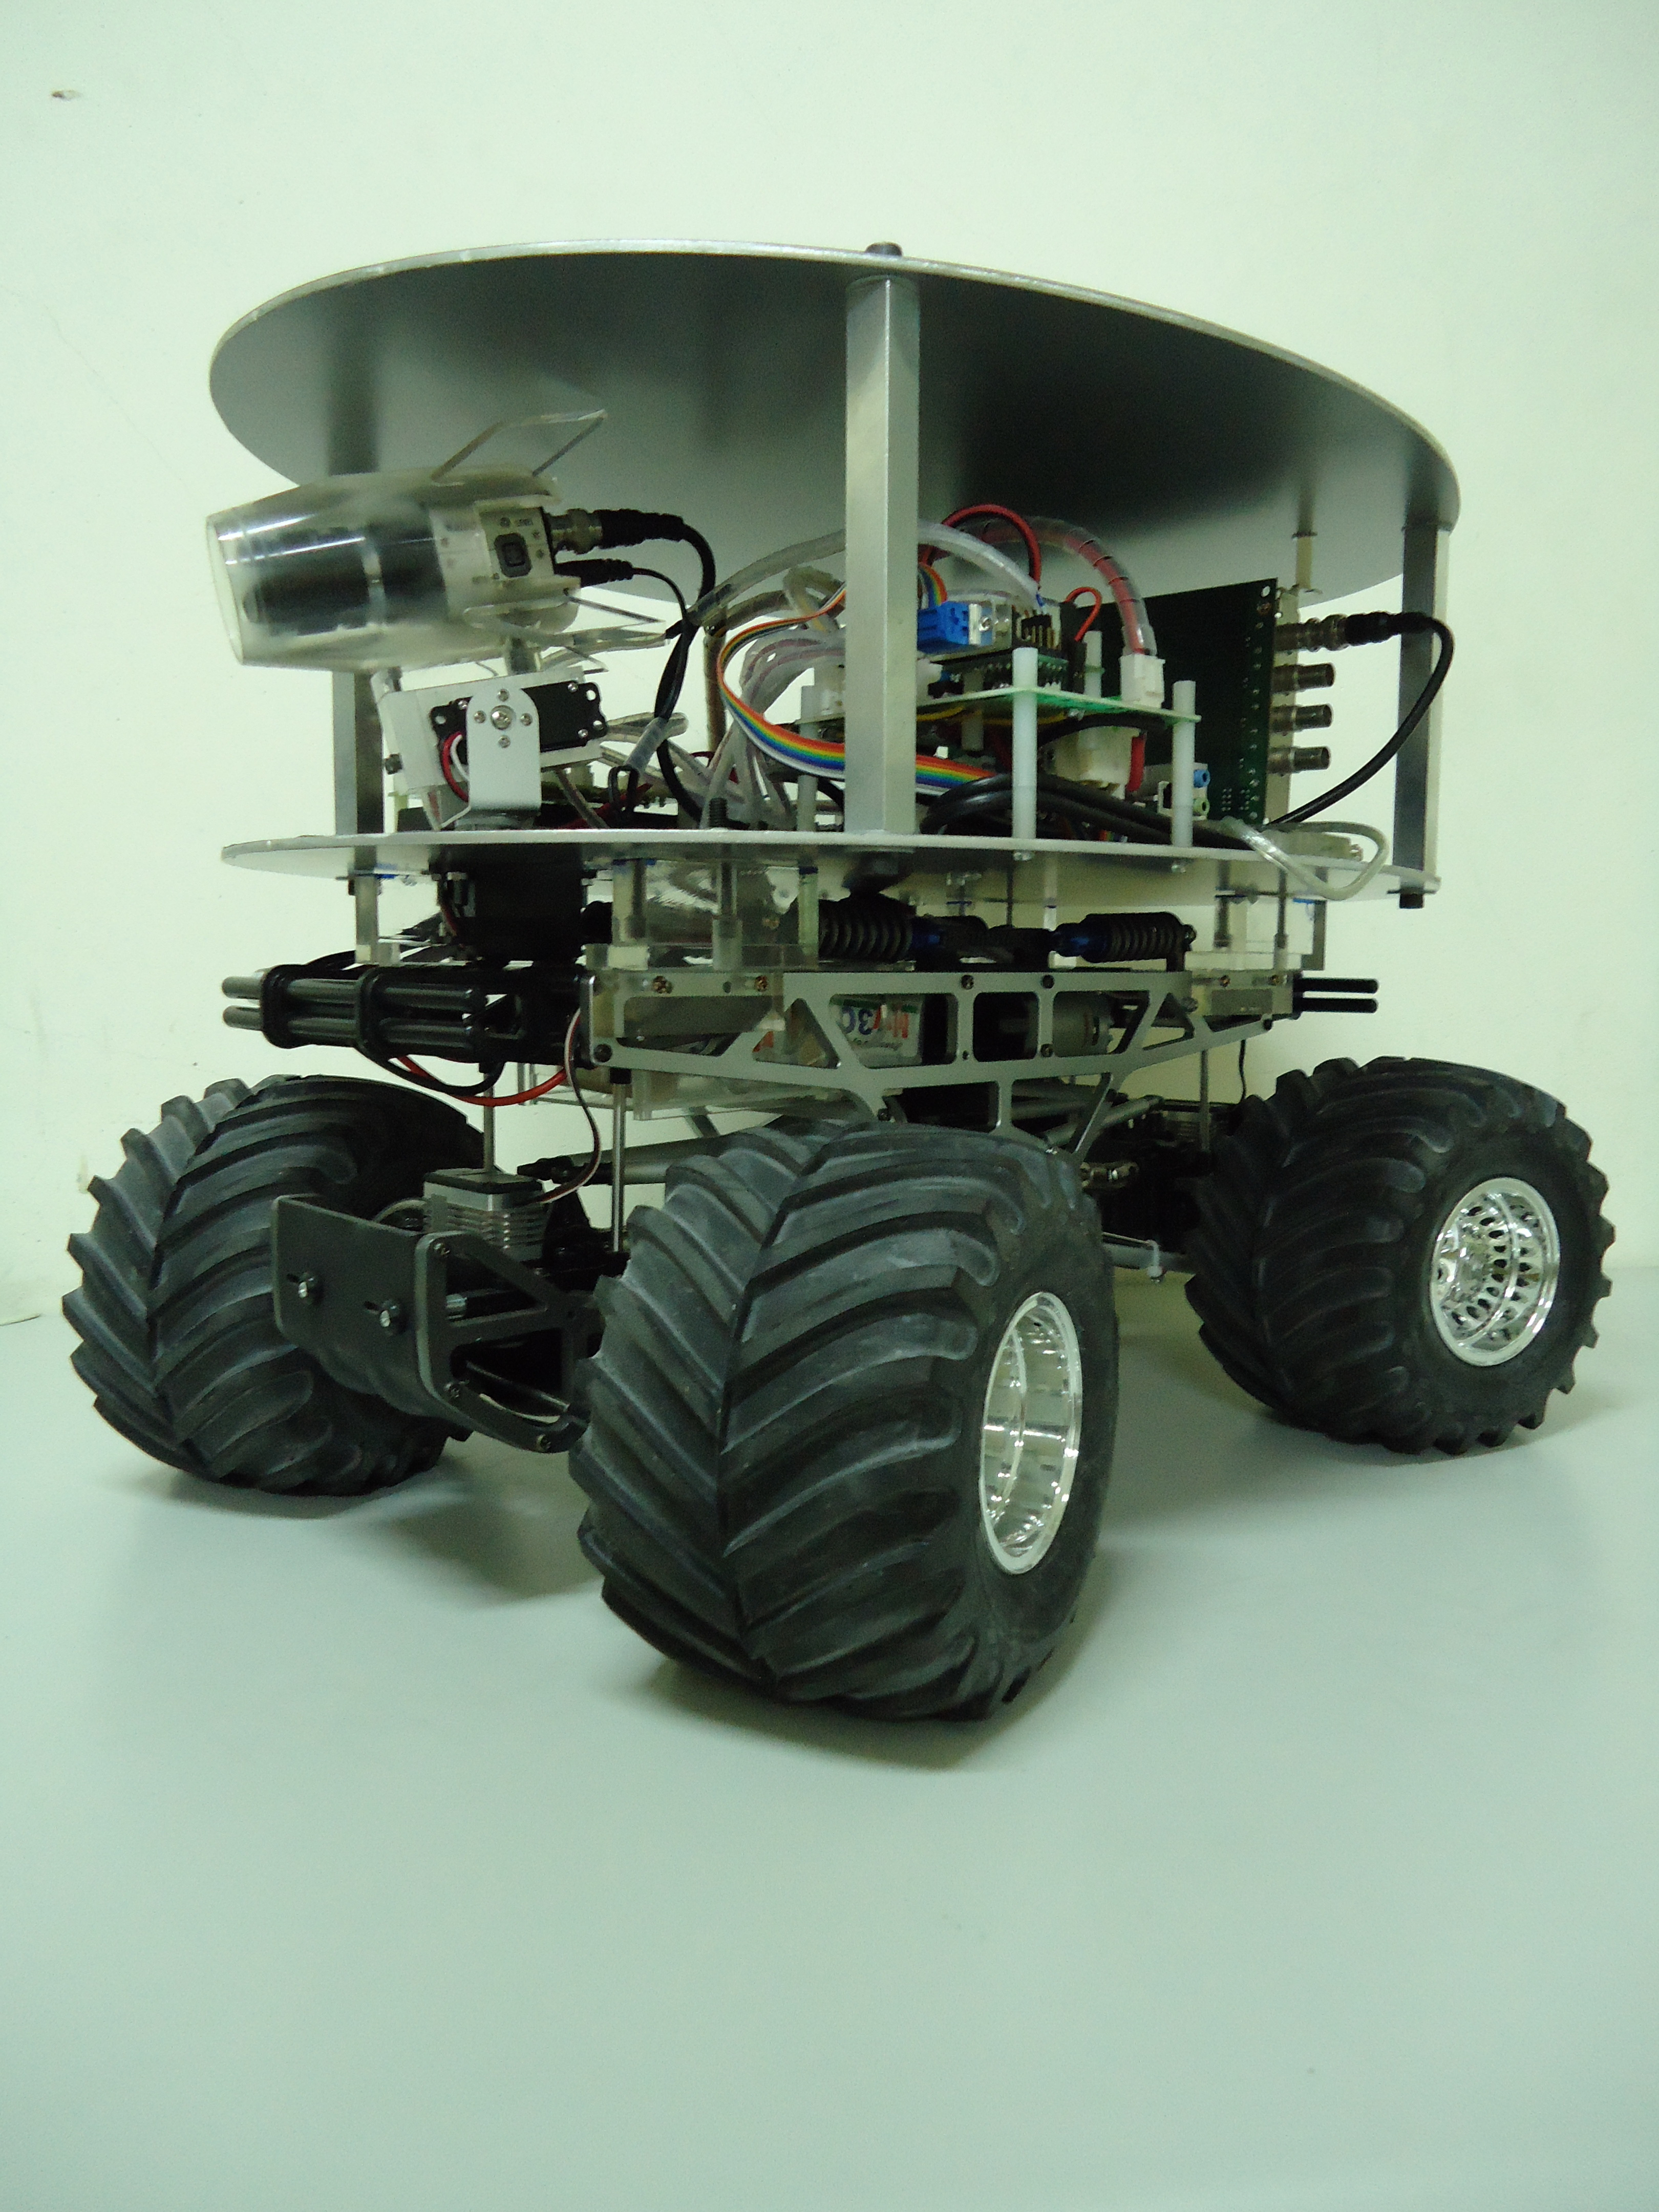
\includegraphics[width=\textwidth]{figures/YunTrooper.jpg}
		\caption{Yun Trooper}
		\label{fig:YunTrooperI}
	\end{subfigure}
	\begin{subfigure}[b]{0.45\textwidth}
		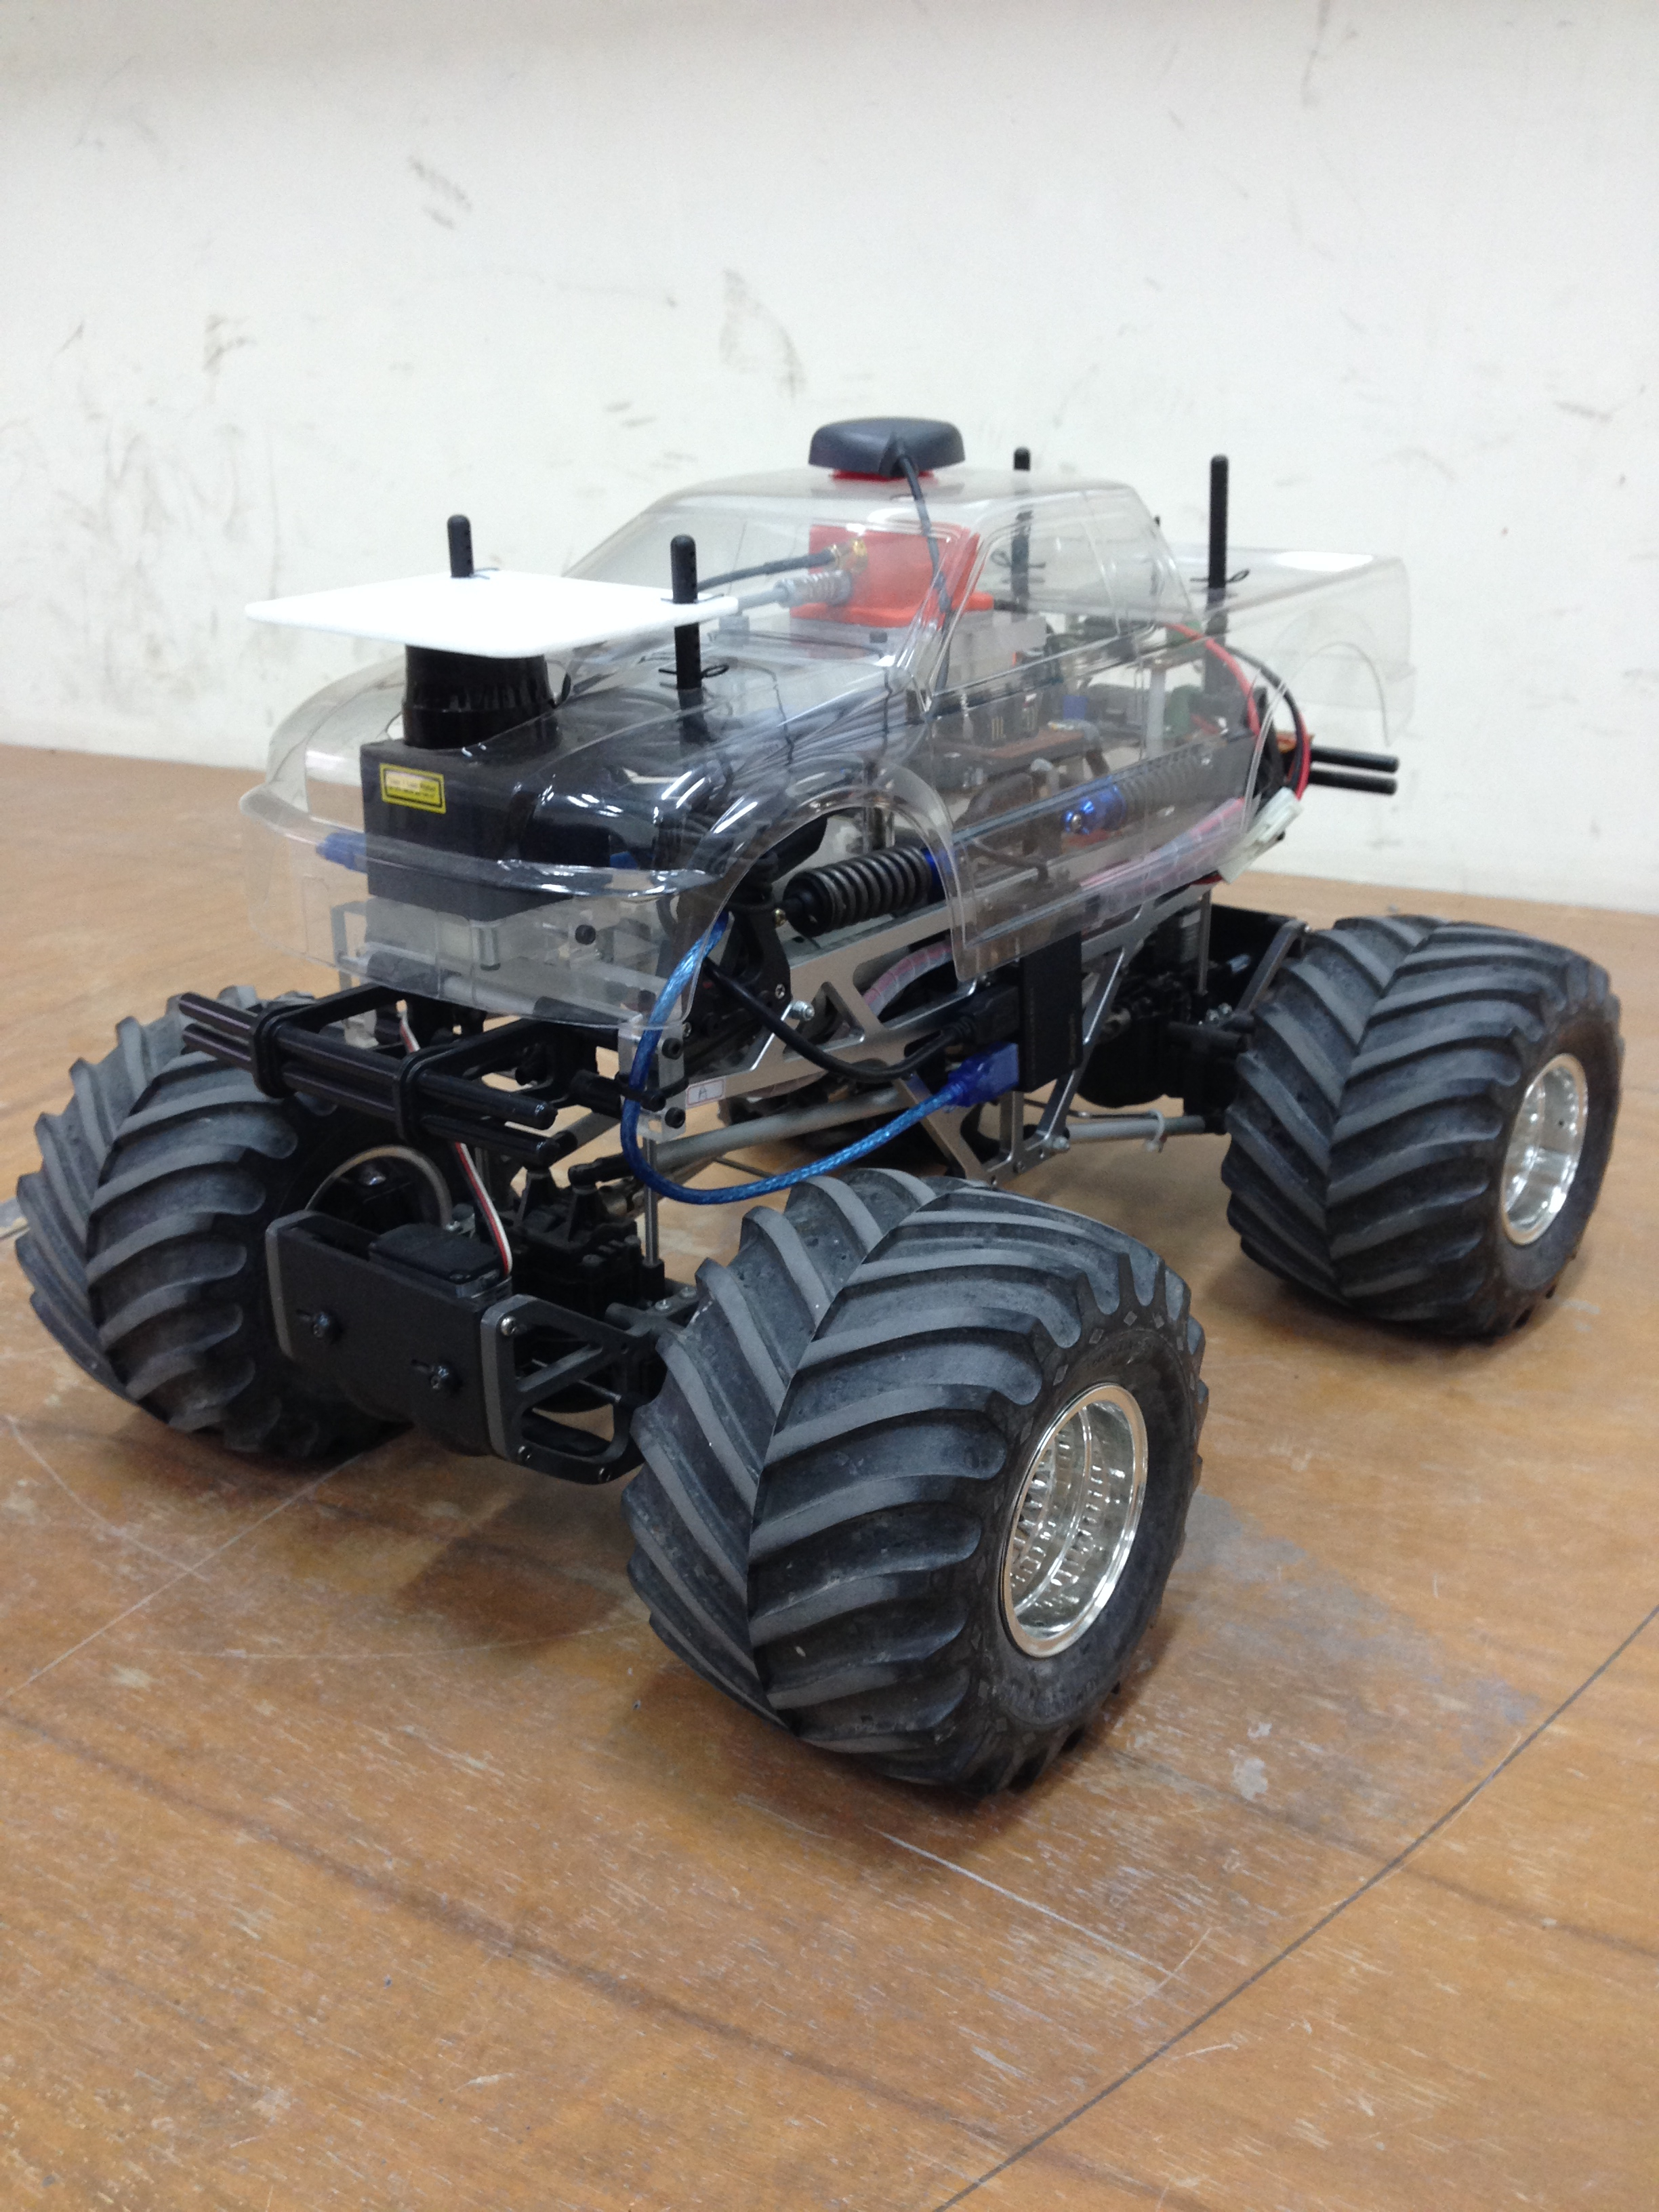
\includegraphics[width=\textwidth]{figures/YunTrooperII.jpg}
		\caption{Yun Trooper II}
		\label{fig:YunTrooperII}
	\end{subfigure}
	\caption{Yun Trooper比較}
\end{figure}

\section{文獻回顧}
這邊就是文獻回顧哩!

\begin{comment}
\section{這是1-1章}
這邊是1-1節!根據\cite{Borenstein:1991:VFH}的說法,這邊就是這個那個這個那個…
但根據\cite{Ulrich:1998:VFHPlus}的說法,這邊應該是…
不過根據\cite{Siegwart:2004:IAMR}的說法,他覺得…

\newpage
\section{這是1-2章}
這邊是1-2節!試著放個圖:
\begin{figure}[h!]
\centering
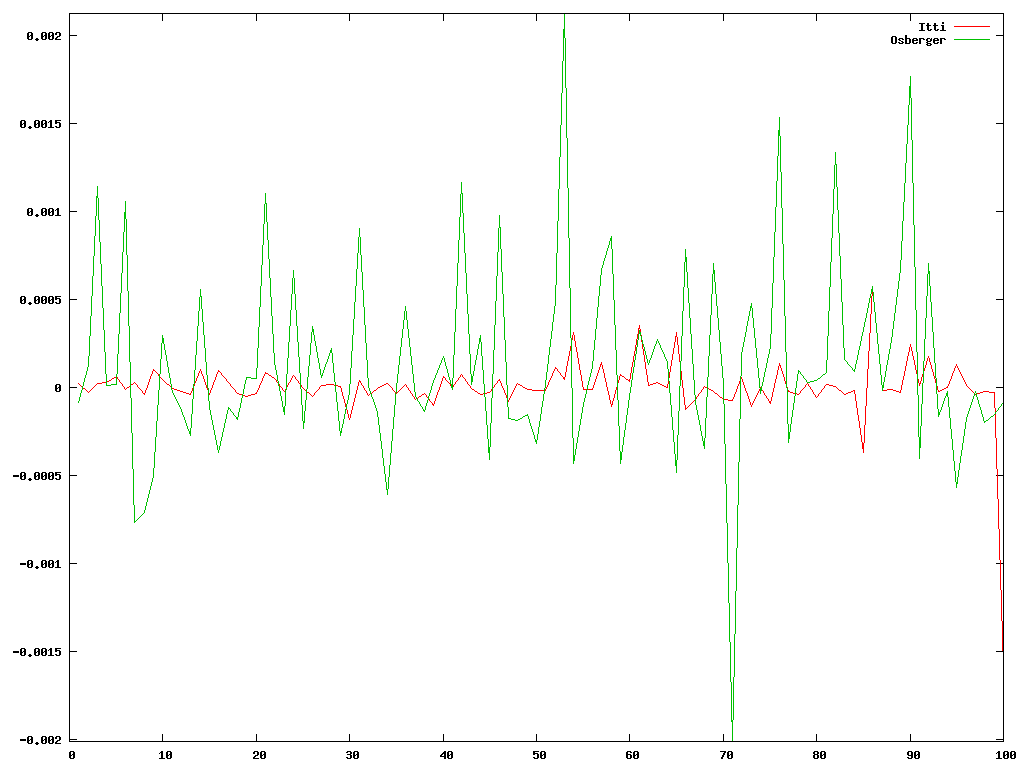
\includegraphics[width=0.45\textwidth]{sample}
\caption{這是範例圖}
\label{kl}
\end{figure}

再試著放個表:
\begin{table}[h!]
\begin{center}
\begin{tabular}{lcc}

\hline
                    &  {\small Itti's method}     & {\small Fuzzy growing}    \\
\hline
{\small Precision}           &  0.4475    & 0.4506 \\
{\small Recall}              &  0.5515    & 0.5542 \\
\hline

\end{tabular}
\caption{這是範例表}
\label{t:FOA}
\end{center}
\end{table}

就這樣啦!
\end{comment}
